\documentclass{article}
\usepackage{amsthm}
\usepackage[dvipsnames]{xcolor}
\usepackage{avant}
\usepackage{fancyhdr}
\usepackage{tikz}
\usetikzlibrary{shapes}
\usepackage{hyperref}
\usepackage[bottom]{footmisc}

\renewcommand{\familydefault}{\sfdefault}   % cambio font
\theoremstyle{definition}
\newtheorem*{definition}{Definizione}
\renewcommand{\figurename}{Figura}
\renewcommand{\contentsname}{Contenuti}

\pagestyle{fancy}
\fancyfoot[L]{Basi di Dati}
\fancyfoot[C]{\thepage}
\fancyfoot[R]{Angelo Passarelli}

\setcounter{section}{-1}

\title{Basi di Dati}
\author{Angelo Passarelli}
\date{\today}

\begin{document}    
    \maketitle
    \begin{center}
        
\includegraphics[scale=0.15]{img/Stemma_unipi.png}
    \end{center}
    \vspace{1cm}
    \begin{center}
        Appunti basati sulle lezioni e dispense della professoressa Giovanna Rosone \footnote{\url{https://pages.di.unipi.it/rosone/index.html}}
    \end{center}
    \pagebreak
    \tableofcontents
    \pagebreak

    \begin{sloppypar}

    \section{Introduzione}

    \begin{definition}[Base di Dati]
        Una base di dati è un insieme organizzato di dati utilizzati per il supporto allo svolgimento di attività.
    \end{definition}

    \paragraph*{Struttura dei Dati}
    I dati sono organizzati in insiemi strutturati che possono presentare fra loro delle relazioni. Tuple che rappresentano dati nello stesso insieme devono essere omogenee ed univoche.

    \begin{definition}[Sistema Informativo]
        Un sistema informativo è una combinazione di risorse umane e/o materiali e procedure organizzate per
        la \textcolor{purple}{raccolta}, l'\textcolor{purple}{archiviazione}, l'\textcolor{purple}{elaborazione}
        e lo \textcolor{purple}{scambio} di informazioni necessarie ad un'attività, le quali possono essere classificate in:
        \begin{itemize}
            \item Informazioni di servizio (operative).
            \item Informazioni di controllo (pianificazione e gestione).
            \item Informazioni di governo (pianificazione strategica).
        \end{itemize}
        \begin{figure}[h]
            \centering
            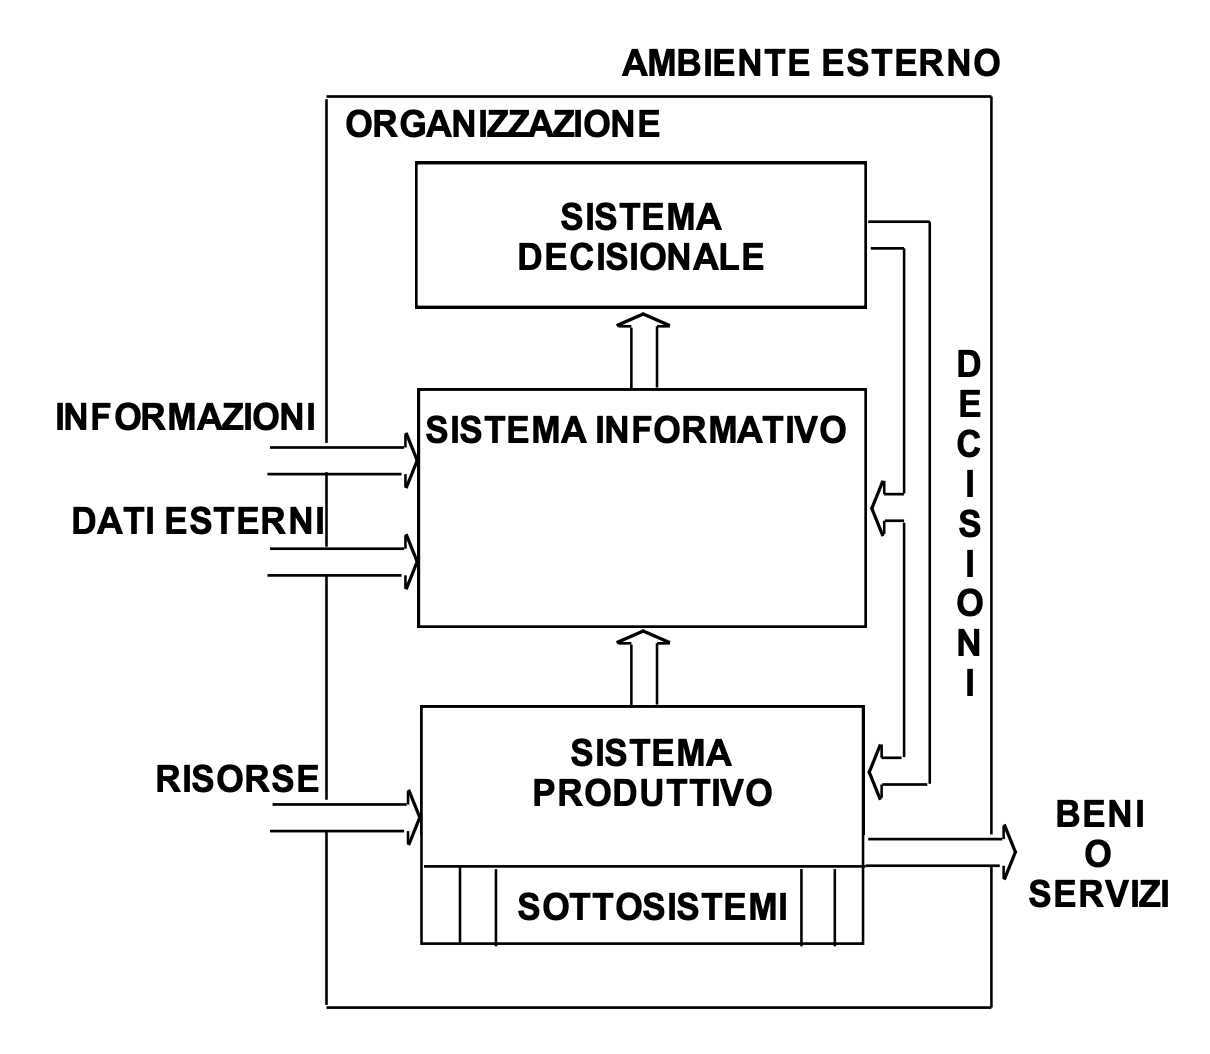
\includegraphics[scale=0.5]{img/sistema_informativo.png}
            \caption{Esempio di sistema informativo}
        \end{figure}
    \end{definition}

    \begin{definition}[Sistema Informativo Automatizzato]
        Un sistema informativo automatizzato è una parte del sistema informativo che permette di implementare le procedure
        che si occupano della gestione delle informazioni usando un sistema informatico.
    \end{definition}

    \begin{definition}[Sistema Informatico]
        Un sistema informatico è l'insieme delle tecnologie a supporto per le attività di un'organizzazione.
        Si possono classificare in:
        \begin{itemize}
            \item \textbf{\textcolor{purple}{Sistemi informatici operativi}}: questi sistemi si utilizzano per svolgere le normali attività dell'azienda
                per la fruizione del suo bene o servizio, e per la gestione interna dei singoli reparti dell'azienda.
                Le operazioni sui dati in questo sistema sono di tipo \textcolor{purple}{OLTP} (\emph{On-Line Transaction Processing})
                e prevedono elaborazioni semplici che coinvolgono pochi dati che vengono aggiornati molto frequentemente.
            \item \textbf{\textcolor{purple}{Sistemi informatici direzionali}}: i dati sono organizzati in \emph{Data Warehouse}
                che consentono di aiutare l'azienda nei processi di controllo delle prestazioni e di decisione manageriale.
                Le elaborazioni su questo tipo di sistema si chiamano \textcolor{purple}{OLAP} (\emph{On-Line Analytical Processing})
                e prevedono l'utilizzo di una grande mole di dati che sono per lo più storici. In questo caso i dati vengono aggiornati
                molto raramente, ma su di essi vengono svolte molte operazioni, anche da un punto di vista multidimensionale, ovvero
                vengono incrociati più dati per analizzare le informazioni ottenute sotto molteplici punti di vista.
        \end{itemize}
    \end{definition}

    \begin{definition}[DBMS]
        Un \emph{Database Management System} è un sistema che garantisce
        il controllo e la gestione di dati per renderli accessibili agli utenti opportuni in base ai loro privilegi.
        Il DBMS fornisce anche dei linguaggi che permettono di definire lo \textcolor{purple}{schema} di un database, di scegliere le \textcolor{purple}{strutture dati}
        opportune per la memorizzazione dei dati, di rispettare i \textcolor{purple}{vincoli} per ogni tipo di dato e di poter \textcolor{purple}{modificare} e
        \textcolor{purple}{interrogare} il database.
    \end{definition}

    \paragraph*{Metadati} All'interno del database sono anche memorizzati dei metadati che si riferiscono agli utenti
    e allo schema utilizzato dal database stesso. Anche i metadati possono essere interrogati e modificati.
    \section{DBMS e Linguaggi}
Si distinguono tre diversi livelli di descrizione dei dati:
\begin{itemize}
    \item A livello di \textcolor{purple}{\emph{vista} logica}: descrive come deve apparire il database a seconda dell'utente che lo usa, in base ai suoi permessi.
    \item A livello \textcolor{purple}{logico}: descrive la struttura degli insiemi dei dati e le relazioni fra essi,
        senza doversi occupare della loro organizzazione nella memoria.
    \item A livello \textcolor{purple}{fisico}: viene descritto come sono organizzati fisicamente i dati nella memoria e
        vengono riportate quali strutture dati ausiliare vengono utilizzate.
\end{itemize}

\begin{center}
    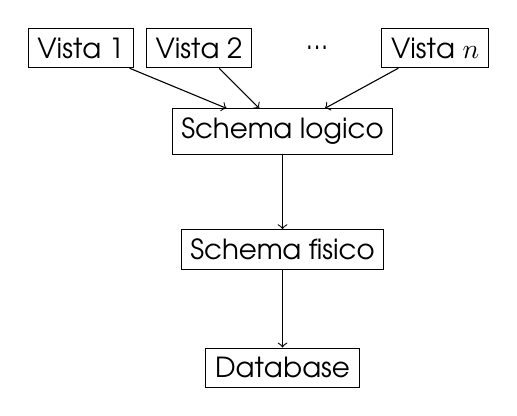
\begin{tikzpicture}[node distance = 1.5cm, main/.style={rectangle, draw}]
        \node[main] (1) {Vista 1};
        \node[main] (2) [right of=1] {Vista 2};
        \node[main, draw opacity=0] (3) [right of=2] {...};
        \node[main] (4) [right of=3] {Vista $n$};
        \node[main] (5) [below right of=2] {Schema logico};
        \node[main] (6) [below of=5] {Schema fisico};
        \node[main] (7) [below of=6] {Database};
        \draw[->] (1) -- (5);
        \draw[->] (2) -- (5);
        \draw[->] (4) -- (5);
        \draw[->] (5) -- (6);
        \draw[->] (6) -- (7);
    \end{tikzpicture}
\end{center}

Quest approccio permette di garantire le proprietà di indipendenza logica e fisica:
\begin{itemize}
    \item \textbf{\textcolor{purple}{Indipendenza Logica}}: gli applicativi non necessitano modifiche in seguite a variazioni dello schema logico.
    \item \textbf{\textcolor{purple}{Indipendenza Fisica}}: gli applicativi non necessitano modifiche in seguito a cambiamenti dell'organizzazione fisica dei dati.
\end{itemize}

Per quanto riguarda i linguaggi di interrogazione, questi possono essere distinti in:
\begin{itemize}
    \item \textbf{\textcolor{purple}{DML}} (Data Manipulation Language): per l'interrogazione e l'aggiornamento dei dati.
    \item \textbf{\textcolor{purple}{DDL}} (Data Definition Language): per la definizione di schemi, sia logici che fisici, ed altre operazioni. 
\end{itemize}

\subsection{Funzionalità del DBMS}
Un DBMS deve prevedere più modalità d'uso per soddisfare le esigenze di più categorie di utenti
che accedono al database. Deve poter offrire:

\begin{itemize}
    \item Un'interfaccia grafica per accedere ai dati.
    \item Un linguaggio di interrogazione per gli utenti inesperti (non programmatori).
    \item Un linguaggio di programmazione per chi sviluppa applicazioni, nello specifico deve prevedere
        l'integrazione del \emph{DDL} e del \emph{DML} nel linguaggio ospite.
    \item Un linguaggio per lo sviluppo di interfacce per le applicazioni.
    \item Predisporre per l'\textcolor{purple}{amministratore} strumenti per stabilire i diritti d'accesso ai dati,
        per il ripristino del sistema e per la modifica e la definizione degli schemi logici (sia interno che esterno).
    
\end{itemize}

\subsection{Proprietà dei Database}
Il DBMS permette di garantire al database le seguenti proprietà:
\begin{itemize}
    \item \textcolor{purple}{Integrità}: mantenimento dei vincoli d'integrità dichiarati in fase di definizione dello schema.
    \item \textcolor{purple}{Affidabilità}: protezione dei dati da parte di malfunzionamenti sia software che hardware e da anomalie indesiderate
        come l'accesso concorrente al database da parte di più utenti.
    \item \textcolor{purple}{Sicurezza}: protezione dei dati da parte di utenti non autorizzati.
\end{itemize}

Inoltre un DBMS deve essere in grado di gestire collezioni di dati che siano:
\begin{itemize}
    \item \textcolor{purple}{Grandi}
    \item \textcolor{purple}{Persistenti}: il periodo di vita dei dati è indipendente dai programmi che li utilizzano.
    \item \textcolor{purple}{Condivise}: possono essere usati da programmi diversi.
\end{itemize}

Il DMBS deve essere anche \textcolor{purple}{efficiente} (utilizzando al meglio le risorse in termini di \emph{spazio} e \emph{tempo}) ed \textcolor{purple}{efficace}.

\subsection{Transazioni}

\begin{definition}[Transazione]
    Una transazione è una serie di azioni di lettura e scrittura sulla memoria permanente
    o di elaborazione dati in memoria temporanea. Presenta le seguenti proprietà:
    \begin{itemize}
        \item \textbf{\textcolor{purple}{Atomicità}}: le transizioni che non vanno a buon fine o che vengono abortite
            sono trattate come se non fossero mai state eseguite.
        \item \textbf{\textcolor{purple}{Persistenza}}: le modifiche effettuate da una transizione andata a buon fine sono permanenti,
            ovvero non possono essere alterate da malfunzionamenti.
        \item \textbf{\textcolor{purple}{Serializzabilità}}: nel caso di esecuzioni concorrenti di più transazioni, l'effetto ottenuto è quello di un'esecuzione seriale.
    \end{itemize}
\end{definition}

\section{Modellazione}
\begin{definition}[Modello Astratto]
    Un modello astratto è la rappresentazione formale di idee e conoscenze relative ad un fenomeno.
\end{definition}

La modellazione è centrale nella progettazione del database che comprende le fasi presenti in figura.
\begin{center}
    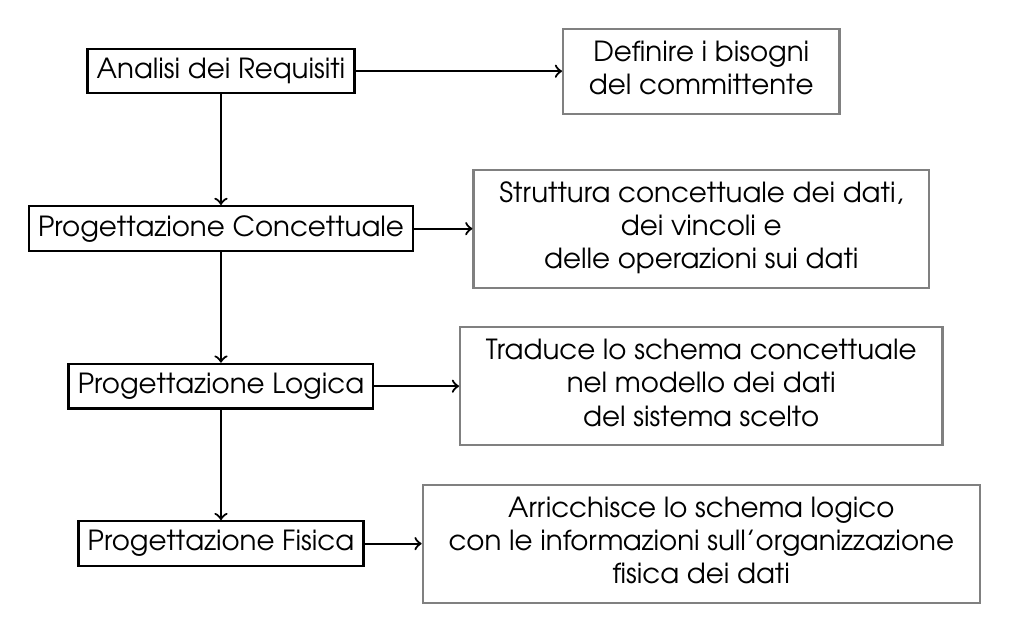
\begin{tikzpicture}[thick, main/.style = {draw, rectangle}, desc/.style = {draw=gray, rectangle}]
        \node[main] (1)  {Analisi dei Requisiti};
        \node[main] (2) [below of=1, node distance = 2cm] {Progettazione Concettuale};
        \node[main] (3) [below of=2, node distance = 2cm] {Progettazione Logica}; 
        \node[main] (4) [below of=3, node distance = 2cm] {Progettazione Fisica};
        \node[desc] (5) [right of=1, node distance = 6.1cm] {\begin{tabular}{c} Definire i bisogni \\ del committente \end{tabular}};
        \node[desc] (6) [below of=5, node distance = 2cm] {\begin{tabular}{c} Struttura concettuale dei dati, \\ dei vincoli e \\ delle operazioni sui dati \end{tabular}};
        \node[desc] (7) [below of=6, node distance = 2cm] {\begin{tabular}{c} Traduce lo schema concettuale \\ nel modello dei dati \\ del sistema scelto \end{tabular}};
        \node[desc] (8) [below of=7, node distance = 2cm] {\begin{tabular}{c} Arricchisce lo schema logico \\ con le informazioni sull'organizzazione \\ fisica dei dati \end{tabular}};
        \draw[->] (1) -- (2);
        \draw[->] (2) -- (3);
        \draw[->] (3) -- (4);
        \draw[->] (1) -- (5);
        \draw[->] (2) -- (6);
        \draw[->] (3) -- (7);
        \draw[->] (4) -- (8);
    \end{tikzpicture}
\end{center}

\subsection{Fasi della Modellazione}

\begin{center}
    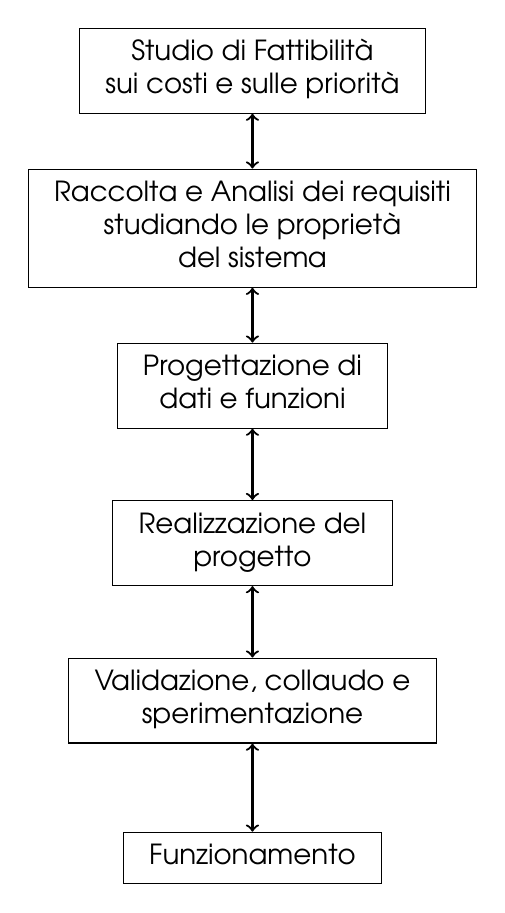
\begin{tikzpicture}[node distance=2cm, main/.style={draw, rectangle}]
        \node[main] (1) {\begin{tabular}{c}Studio di Fattibilità \\ sui costi e sulle priorità\end{tabular}};
        \node[main] (2) [below of=1] {\begin{tabular}{c}Raccolta e Analisi dei requisiti \\ studiando le proprietà \\ del sistema\end{tabular}};
        \node[main] (3) [below of=2] {\begin{tabular}{c}Progettazione di \\ dati e funzioni\end{tabular}};
        \node[main] (4) [below of=3] {\begin{tabular}{c}Realizzazione del \\ progetto\end{tabular}};
        \node[main] (5) [below of=4] {\begin{tabular}{c}Validazione, collaudo e \\ sperimentazione\end{tabular}};
        \node[main] (6) [below of=5] {\begin{tabular}{c}Funzionamento\end{tabular}};
        \draw[<->, thick] (1) -- (2);
        \draw[<->, thick] (2) -- (3);
        \draw[<->, thick] (3) -- (4);
        \draw[<->, thick] (4) -- (5);
        \draw[<->, thick] (5) -- (6);
    \end{tikzpicture}   
\end{center}

\subsection{Analizzare il Dominio}
Il dominio può presentare più aspetti da dover analizzare:
\begin{itemize}
    \item Aspetto \emph{\textcolor{purple}{ontologico}}: conoscere ciò che si suppone esista nell'universo del contesto e quindi ciò che è da modellare.
        Occorre analizzare tre tipi di conoscenze:
        \begin{itemize}
            \item Conoscenza \emph{\textcolor{purple}{concreta}}: le entità del contesto e le associazioni fra di esse.
                \begin{definition}[Entità]
                    Sono oggetti di cui occorre definire le proprietà.
                \end{definition}
                \begin{definition}[Proprietà]
                    Descrivono le caratteristiche di determinate entità e sono formata da una coppia \verb+(Attributo, Valore)+.
                    Ogni proprietà ha ad essa associato un dominio, quindi un insieme di valori che può assumere. Inoltre le proprietà si possono classificare in:
                    \begin{itemize}
                        \item \textcolor{purple}{Atomiche} o \textcolor{purple}{Strutturate}: atomiche se il loro valore non è ulteriormente scomponibile.
                        \item \textcolor{purple}{Totali} o \textcolor{purple}{Parziali}: se è obbligatoria oppure opzionale.
                        \item \textcolor{purple}{Univoche} o \textcolor{purple}{Multivalore}: univoca se per ogni entità la scelta del valore è unico (\emph{es. codice fiscale}).
                        \item \textcolor{purple}{Costanti} o \textcolor{purple}{Variabili}
                        \item \textcolor{purple}{Calcolate} o \textcolor{purple}{Non Calcolate}: calcolata se è possibile derivarla da altre proprietà.
                    \end{itemize}
                \end{definition}
                \begin{definition}[Tipo di un'entità]
                    Ogni entità appartiene ad un tipo che ne indica la propria natura.
                \end{definition}
                \begin{definition}[Collezione]
                    Insieme di entità dello stesso tipo.
                \end{definition}
            \item Conoscenza \emph{\textcolor{purple}{astratta}}: la struttura e i vincoli sulle entità.
            \item Conoscenza \emph{\textcolor{purple}{procedurale}}: le operazioni di base, sia dei singoli utenti e sia come avviene la comunicazione con il sistema informatico.
        \end{itemize}
    \item Aspetto \emph{\textcolor{purple}{logico}}: meccanismi di astrazione (\emph{modello di dati, per es. diagrammi E-R \footnote{\url{https://it.wikipedia.org/wiki/Modello_E-R}}}) con cui descrivere la struttura della conoscenza concreta.
    \item Aspetto \emph{\textcolor{purple}{linguistico}}: linguaggio formale con cui definire il modello.
    \item Aspetto \emph{\textcolor{purple}{pragmatico}}: insieme di regole da seguire in fase di modellazione.
\end{itemize}

\subsection{Oggetti e Classi}

\begin{definition}[Oggetto]
    Un oggetto è un'entità software che presenta uno \emph{stato}, un \emph{comportamento} e un'\emph{identità}.
    Lo \textcolor{purple}{stato} è rappresentato da un insieme di costanti o variabili, mentre il \textcolor{purple}{comportamento} è un
    insieme di procedure locali chiamate \emph{metodi}.
    Un oggetto può rispondere a dei messaggi di input, con dei valori memorizzati nello stato o
    calcolandoli con un metodo.
\end{definition}

\begin{definition}[Classe]
    Una classe è un insieme di oggetti dello stesso tipo, e presenta delle operazioni per l'inserimento
    e la rimozione di elementi.
\end{definition}

\begin{definition}[Tipo Oggetto]
    Un tipo oggetto definisce l'insieme degli attributi a cui può combaciare
    un insieme di possibili oggetti. I tipi oggetto non sono presenti nei diagrammi E-R,
    però dagli attributi di una collezione è possibile dedurre il tipo oggetto associato.
\end{definition}
    \subsection{Associazioni}

\begin{definition}[Istanza di un'associazione]
    Un'istanza di un'associazione determina un legame logico tra due o più istanze.
\end{definition}

\begin{definition}[Associazione]
    Un'associazione $R(X, Y)$ fra due collezioni di entità chiamate $X$ e $Y$
    è un insieme, che varia nel tempo, di istanze di associazione tra gli elementi delle due collezioni.
    Il prodotto cartesiano $(X \cdot Y)$ è chiamato \textcolor{purple}{dominio dell'associazione}.
\end{definition}

Un'associazione è caratterizzata da due proprietà: \textcolor{purple}{molteplicità} e \textcolor{purple}{totalità}.

\begin{definition}[Vincolo di Unicità]
    Un'associazione $R(X, Y)$ è detta \textcolor{purple}{univoca}
    rispetto ad $X$ se per ogni elemento di $x \in X$ esiste al più un elemento
    $y \in Y$ che è associato ad $x$. Se questo vincolo non vale, si dice che l'associazione
    è \textcolor{purple}{multivalore} rispetto ad $X$.
\end{definition}

\paragraph{Cardinalità dell'Associazione}

\begin{itemize}
    \item $R(X, Y)$ è \textbf{\textcolor{purple}{(1:N)}} se è multivalore sy $X$ ed univoca su $Y$.
    \item $R(X, Y)$ è \textbf{\textcolor{purple}{(N:1)}} se è univoca sy $X$ e multivalore su $Y$.
    \item $R(X, Y)$ è \textbf{\textcolor{purple}{(N:M)}} se è multivalore sy $X$ e multivalore su $Y$.
    \item $R(X, Y)$ è \textbf{\textcolor{purple}{(1:1)}} se è univoca sy $X$ ed univoca su $Y$.
\end{itemize}

\begin{definition}[Vincolo di Totalità]
    Un'associazione $R(X, Y)$ è detta \textcolor{purple}{totale} su X se per ogni elemento
    $x \in X$ esiste almeno un elemento $y \in Y$ associato ad $x$. Se questo vincolo non vale,
    si dice che l'associazione è \textcolor{purple}{parziale} rispetto ad $X$.
\end{definition}

\newpage
\paragraph{Rappresentazione delle Associazioni} Un'associazione fra due collezioni $C_1$ e $C_2$ si rappresenta
con una linea che collega le due classi. La linea si etichetta con il nome dell'associazione. L'\textcolor{purple}{univocità}
di una classe $C_1$ si rappresenta disegnando una freccia singola sulla linea che esce và da $C_1$ a $C_2$. Se invece l'associazione è
\textcolor{purple}{multivalore} si indica con una doppia freccia.
La \textcolor{purple}{parzialità} invece è rappresentata con un taglio sulla linea vicino alla freccia, mentre la
\textcolor{purple}{totalità} è rappresentata dall'assenza del taglio.

\begin{figure}[h]
    \centering
    \captionsetup{justification=centering}
    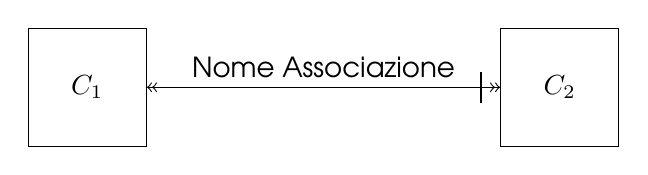
\begin{tikzpicture}[node distance=6cm, scale=2, main/.style={rectangle, draw, minimum size=15mm}]
        \node[main] (1) {$C_1$};
        \node[main] (2) [right of=1]{$C_2$};
        \draw[<<->>] (1) -- (2) node[midway, above] {Nome Associazione};
        \draw (2.5, 0.1) -- (2.5, -0.1);
    \end{tikzpicture}
    \caption{In questo caso abbiamo un'associazione \emph{multivalore} da entrambe la parti, ma \emph{parziale} per $C_2$ e \emph{totale} per $C_1$}
\end{figure}

\begin{figure}[h]
    \centering
    \captionsetup{justification=centering}
    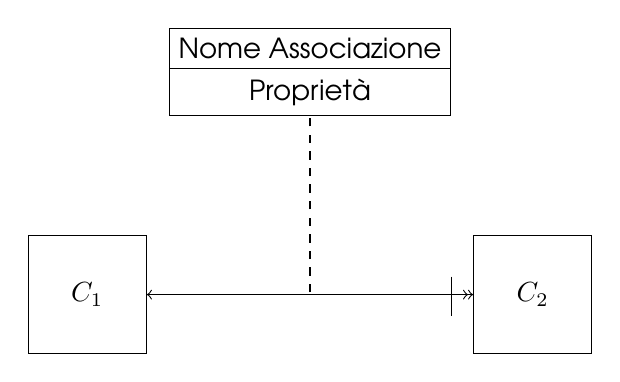
\begin{tikzpicture}[node distance=4cm, scale=2, main/.style={rectangle, draw, minimum size=15mm}]
        \node[rectangle split, rectangle split parts=2, draw] (prop) {Nome Associazione \nodepart{second} Proprietà};
        \node[main] (1) [below left of=prop]{$C_1$};
        \node[main] (2) [below right of=prop]{$C_2$};
        \draw[<->>] (1) -- (2);
        \draw (0.9, -1.3) -- (0.9, -1.55);
        \draw[dashed] (0, -1.4) -- (prop);
    \end{tikzpicture}
    \caption{Le associazioni possono presentare \textcolor{purple}{proprietà}}
\end{figure}

\begin{figure}[h]
    \centering
    \captionsetup{justification=centering}
    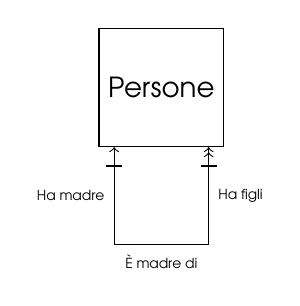
\begin{tikzpicture}[node distance=4cm, scale=2, main/.style={rectangle, draw, minimum size=15mm}]
        \node[main] (1) {Persone};
        \draw[->] (-0.3, -1) -- (-0.3, -0.38) node[midway, left] {\tiny{Ha madre}};
        \draw[->>] (0.3, -1) -- (0.3, -0.38) node[midway, right] {\tiny{Ha figli}};
        \draw[-] (-0.3, -1) -- (0.3, -1) node[midway, below] {\tiny{È madre di}};
        \draw[-] (-0.35, -0.5) -- (-0.25, -0.5);
        \draw[-] (0.25, -0.5) -- (0.35, -0.5);
    \end{tikzpicture}
    \caption{O possono anche essere \textcolor{purple}{ricorsive}. In questo caso occorre etichettare l'associazione non solo con il proprio nome, ma anche con i nomi dei ruoli che hanno le due entità nell'associazione.}
\end{figure}

\paragraph{\textcolor{purple}{Associazione Non Binarie}}
Le associazioni non binarie, per semplicità, non vengono rappresentate graficamente, ma ad esempio,
per quanto riguarda quelle \emph{ternarie}, queste vengono trasformate in tre associazioni \emph{binarie} aggiungendo un'altra
collezione al posto dell'associazione \emph{ternaria}.

    \end{sloppypar}
\end{document}